\section{System Disk Encryption}
An encrypted system disk, prevents that the data contained in it can be clone or replicated without the passphrase or authentication server. For this design, the disks will be encrypted through kickstart passphrase and then removed once the remote Tang server are reached, which means, of non-authorized user gains physical access to the server:
\begin{itemize}
  \item Once the server boots, it will require root credentials.
  \item If halted and attempt to change the root password, the encryption passphrase prompt will be requested - which was deleted.
  \item If booted through a Live USB OS, the encrypted partitions remain unreadable.
  \item If the drive is taken, the disk would never gain access to its content.
\end{itemize}
\newpage
\subsection{LUKS - Linux Unified Key Setup}
According to a paper subscribed by Danut Anton an Emil Simion \footnote[1]{https://ieeexplore-ieee-org.usm.idm.oclc.org/stamp/stamp.jsp?tp=\&arnumber=8678978}, LUKS is one of the most common FDE solution for Linux based systems.
FDE works by encrypting every single bit on a storage device, so if the user doesn't have the password, data cannot be recovered. The most common problem for FDE solutions is password management, which at what concerns this implementation, will be handled by a two level key hierarchy. A strong master key is generated by an OS, which is used for encrypt/decrypt the hard drive. That key has to be split and encrypted with secret user key and stored on the device, at the beginning of the memory. The advantage of this approach is that you can have multiple systems with multiple keys, allowing you to have multiple decryption Servers.
\vskip 2cm
\begin{figure}
  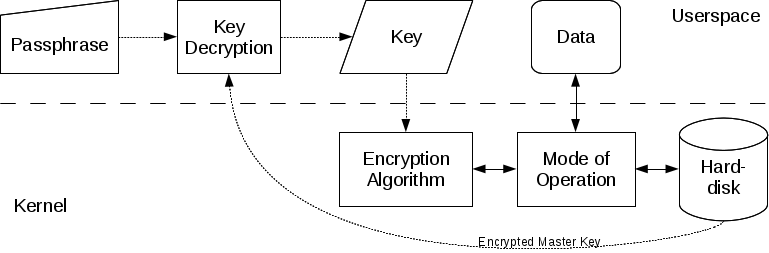
\includegraphics[width=14cm]{images/image2.png}
  \centering
  \caption{LUKS Operational Diagram}
\end{figure}

\newpage
\subsection{Clevis Service}

\newpage
\subsection{Clevis Puppet Profile and Role}


\newpage
\section{Tang Server - Decryption Agent}

\subsection{Tang Puppet Profile and Role}

\newpage
\section{Lab Testing - Proof of Concept}
\subsection{Testing Criteria}
\subsection{Lab Results}
\subsection{Conclusions}
\newpage